\documentclass[10pt,twocolumn]{article}
\usepackage[margin=0.75in]{geometry}
\setlength{\columnsep}{0.28in}
\usepackage{amsmath,amssymb}
\usepackage{booktabs}
\usepackage{graphicx}
\usepackage{microtype}
\usepackage[table]{xcolor}
\usepackage{tikz}
\usetikzlibrary{arrows.meta,positioning,fit,backgrounds}
\usepackage[colorlinks=true,allcolors=blue!55!black]{hyperref}
\usepackage{caption}
\captionsetup{font=small,labelfont=bf,skip=4pt}
\setlength{\emergencystretch}{2em}

% Tighter heading spacing. The default \paragraph leaves 3.25ex above every
% run-in heading, and this report has a dozen of them.
\usepackage{titlesec}
\titlespacing*{\section}{0pt}{1.6ex plus .3ex}{0.9ex}
\titlespacing*{\subsection}{0pt}{1.4ex plus .3ex}{0.7ex}
\titlespacing*{\paragraph}{0pt}{1.0ex plus .2ex}{0.6em}

% generated by scripts/make_report_tables.py
\newcommand{\naiveValWape}{52.34}
\newcommand{\naiveTestWape}{49.96}
\newcommand{\seasonalValWape}{37.27}
\newcommand{\seasonalTestWape}{31.38}
\newcommand{\patchValWape}{15.70}
\newcommand{\patchTestWape}{14.47}
\newcommand{\patchEpochs}{2}
\newcommand{\patchParams}{593}
\newcommand{\patchMinutes}{39}
\newcommand{\lstmValWape}{15.92}
\newcommand{\lstmTestWape}{14.71}
\newcommand{\lstmEpochs}{8}
\newcommand{\lstmParams}{416}
\newcommand{\lstmMinutes}{86}
\newcommand{\ensValWape}{15.37}
\newcommand{\ensTestWape}{14.18}
\newcommand{\ensValMae}{1.44}
\newcommand{\ensWeight}{0.55}
\newcommand{\ensVsNaive}{72}
\newcommand{\ensVsSeasonal}{59}
\newcommand{\gapValWape}{15.40}
\newcommand{\lstmRevinValWape}{18.42}
\newcommand{\lstmRevinTestWape}{24.09}
\newcommand{\patchRevinValWape}{15.92}
\newcommand{\patchRevinTestWape}{15.56}


\title{\vspace{-2.2em}Known-Future Covariates Are the Signal:\\A Patch Transformer with Covariate Query Tokens\\for Multivariate Operational Load Forecasting\vspace{-0.4em}}
\author{Group ID: 140 \\ Rosela Berberi, Anja Koroveshi \\ \small Deep Learning (SS26) bonus project, TU Darmstadt}
\date{}

\begin{document}
\twocolumn[
  \begin{@twocolumnfalse}
  \maketitle
  \begin{abstract}
  \noindent
  We forecast a $336$-hour horizon for $96$ correlated operational load series from
  a $168$-hour history and $22$ covariates. Our central observation is that on this
  benchmark the covariates are \emph{known in advance} for the whole forecast
  window, which shifts the problem from extrapolating the target towards learning a
  covariate-to-load response specific to each unit. We therefore extend the PatchTST
  backbone with \emph{future covariate query tokens}, a per-series embedding and a
  pointwise covariate residual path, and contrast it with an LSTM+Attention
  encoder--decoder that decodes iteratively. On held-out tails of the public
  training data our submitted model reaches \ensValWape\,\% WAPE in the validation
  regime --- \ensVsSeasonal\,\% below the seasonal-mean baseline --- and
  \ensTestWape\,\% in a harder regime reproducing the private split's $336$-step
  unobserved gap, cutting the naive last-value error by \ensVsNaive\,\%. Two of our
  conclusions had to be reversed by experiments, and we report both: the recurrent
  decoder's apparent collapse across the gap
  (\lstmRevinValWape\,\%$\,\rightarrow\,$\lstmRevinTestWape\,\%) turned out to be
  reversible instance normalisation compounding through the rollout rather than
  iterative decoding; and our architecture ranking was an artefact of the compute
  budget, inverting once training was no longer starved. Ablations attribute almost
  all of the remaining gain to the covariate pathway rather than to the backbone,
  and a transfer to Jena Climate, where every channel except the calendar is
  past-only, shows how much of that margin the covariate contract rather than the
  architecture was buying.
  \end{abstract}
  \vspace{0.4em}
  \end{@twocolumnfalse}
]

\section{Introduction}

Multivariate time series forecasting asks for the joint future of several
correlated signals given their shared past. This project's benchmark is an
operational instance: $96$ anonymised units report an hourly \emph{operational load
index} and the task is to predict $336$ hours ahead for each. If the index tracks
pressure on a unit, as its description suggests, such a forecast is what drives
staffing decisions; methodologically it is interesting because the horizon is
$2\times$ the conditioning window, so no part of the answer can be read off the
recent past by persistence.

Our starting point was an empirical look at the released tables rather than at the
model zoo, and it changed the project. The file \texttt{validation\_input.csv}
covers \emph{exactly} the rows of \texttt{forecast\_index\_validation.csv}: all
$22$ covariates are supplied for the forecast window itself, while the target is
withheld. The benchmark is thus not a pure extrapolation task but a
\emph{covariate-conditioned} one, and the strongest covariate correlates $0.68$
with the target at the same hour, whereas the target's own autocorrelation has
already decayed to $0.26$ after six hours. A second measurement shaped the
architecture: a per-series OLS fit on the covariates reaches $17.6$\,\% WAPE
against $22.1$\,\% for a single pooled fit, i.e.\ the covariate-to-load response is
unit-specific even though the static columns barely explain anything.

Two consequences follow: a model should consume the future covariates
\emph{directly} at the resolution at which they act, and it needs a per-unit degree
of freedom. We build both into a PatchTST \cite{nie2023patchtst} backbone and
compare against the recurrent-attention hybrid from our expos\'e. Our contributions
are \textbf{PatchTST-cov}, a patch Transformer whose forecast window enters as
patched \emph{future covariate query tokens}, with a per-series embedding and a
pointwise covariate residual path (Sec.~\ref{sec:method}); a \textbf{gap-aware
protocol} that scores every model both immediately after the history and across the
$336$-step gap separating it from the private test window
(Sec.~\ref{sec:protocol}); an \textbf{ablation study} plus a permutation analysis
of which covariates the model uses (Sec.~\ref{sec:ablations}); and a
\textbf{transfer experiment} on Jena Climate, chosen because it inverts the
covariate contract (Sec.~\ref{sec:jena}).

\section{Related Work}

\paragraph{Recurrent forecasters.} LSTMs \cite{hochreiter1997lstm} underpin
probabilistic forecasters such as DeepAR \cite{salinas2020deepar}, which also
popularised the per-series embedding we adopt, and additive attention
\cite{bahdanau2015attention} lets a decoder re-read all encoder states. Iterative
decoders suffer from \emph{exposure bias}, for which scheduled sampling
\cite{bengio2015scheduled} is the standard mitigation and the one we use.

\paragraph{Transformers for long-horizon forecasting.} After the original
Transformer \cite{vaswani2017attention}, a line of work attacked its quadratic cost
and point-wise tokenisation of time series: Informer's sparse attention
\cite{zhou2021informer}, Autoformer's decomposition and auto-correlation
\cite{wu2021autoformer}, FEDformer's frequency-domain attention
\cite{zhou2022fedformer}. PatchTST \cite{nie2023patchtst} instead tokenises
\emph{sub-series patches} and processes each channel independently with a shared
backbone, preserving local semantics while shortening the sequence by the patch
stride; iTransformer \cite{liu2024itransformer} inverts the axes and attends over
variates. A sceptical counter-line matters for calibration: DLinear
\cite{zeng2023dlinear} showed a single linear layer can match several of these
Transformers, and N-BEATS \cite{oreshkin2020nbeats}, N-HiTS \cite{challu2023nhits}
and TiDE \cite{das2023tide} reach comparable accuracy with MLPs. We take that
seriously: our ablations include a covariate-free variant, so the gain we claim is
attributable to the covariate machinery rather than to attention per se.

\paragraph{Covariate-conditioned models.} The Temporal Fusion Transformer
\cite{lim2021tft} is the closest relative of our design: it separates static,
past-only and known-future inputs and feeds the latter to the decoder; TiDE
\cite{das2023tide} does the same with a dense encoder. We borrow that taxonomy and
contribute a minimal way to graft it onto a patch backbone, as query tokens on the
same token sequence.

\paragraph{Normalisation, regularisation, optimisation.} Reversible instance
normalisation \cite{kim2022revin} is the near-default remedy for distribution shift
between training and forecast windows; Sec.~\ref{sec:ablations} finds it harmful at
this horizon, which is one of our main results. We also use spatial dropout
\cite{tompson2015spatialdropout}, AdamW \cite{loshchilov2019adamw} and cosine
annealing with warm restarts \cite{loshchilov2017sgdr}, in PyTorch
\cite{paszke2019pytorch}; dilated convolutions \cite{bai2018tcn} and deep
state-space models \cite{gu2022s4,gu2024mamba} are the natural next backbones.

\section{Method}
\label{sec:method}

\subsection{Problem setup and features}

For series $i$ and origin $t$ we observe the target history
$y_{i,t-L+1:t} \in \mathbb{R}^{L}$ with $L=168$, encoder covariates
$X^{\mathrm{h}}_{i,t-L+1:t} \in \mathbb{R}^{L \times F_{\mathrm{h}}}$, the
known-future covariates $X^{\mathrm{f}}_{i,t+1:t+H} \in \mathbb{R}^{H \times
F_{\mathrm{f}}}$ and static features $s_i \in \mathbb{R}^{S}$, and predict
$\hat{y}_{i,t+1:t+H}$.

The $22$ released covariates split into six calendar encodings (hour and
day-of-week sine/cosine, a weekend flag, a normalised trend), $13$ exogenous hourly
drivers (demand, staffing, queue and network pressure, event load, maintenance,
several risk indices) and three static columns. Ten drivers are missing at random
for $\approx\!4.5$\,\% of rows; we interpolate within each series and append a
binary \emph{missingness indicator} per affected column, so the network can tell an
imputed value from an observed one. This yields $F_{\mathrm{h}}=F_{\mathrm{f}}=29$
and $S=3$. Covariates are standardised with statistics fitted on the training slice
only and serialised into the checkpoint, so inference reproduces training
preprocessing without the training CSV.

The primary metric is $\mathrm{WAPE} = 100\cdot\sum|y-\hat{y}| / \sum|y|$, whose
denominator is constant for a fixed evaluation set. WAPE is therefore a rescaled sum
of absolute errors, and the aligned objective is plain $L_1$ \emph{in the original
target units}~\cite{hyndman2006measures} --- in particular not on per-window
normalised targets, which would silently reweight series by their own scale.

\subsection{Shared components}

\paragraph{RevIN.} Each window is normalised by its own mean and standard
deviation over time and the prediction is de-normalised with the same statistics
\cite{kim2022revin}. We implement it \emph{statelessly}, passing the statistics
explicitly in both directions, so that the conditioning-window statistics survive
an autoregressive rollout: caching them on the module --- as reference
implementations do --- lets the decoder's own call on a single timestep overwrite
them with $(\mu,\sigma)=(y_t,0)$.

\paragraph{Series embedding.} A learned vector $e_i \in \mathbb{R}^{16}$ per
series is concatenated to $s_i$ \cite{salinas2020deepar}. Row $0$ is reserved for
unseen series, so a checkpoint degrades gracefully rather than failing if the
private split introduces a new unit.

\begin{figure*}[t]
\centering
\resizebox{\textwidth}{!}{%
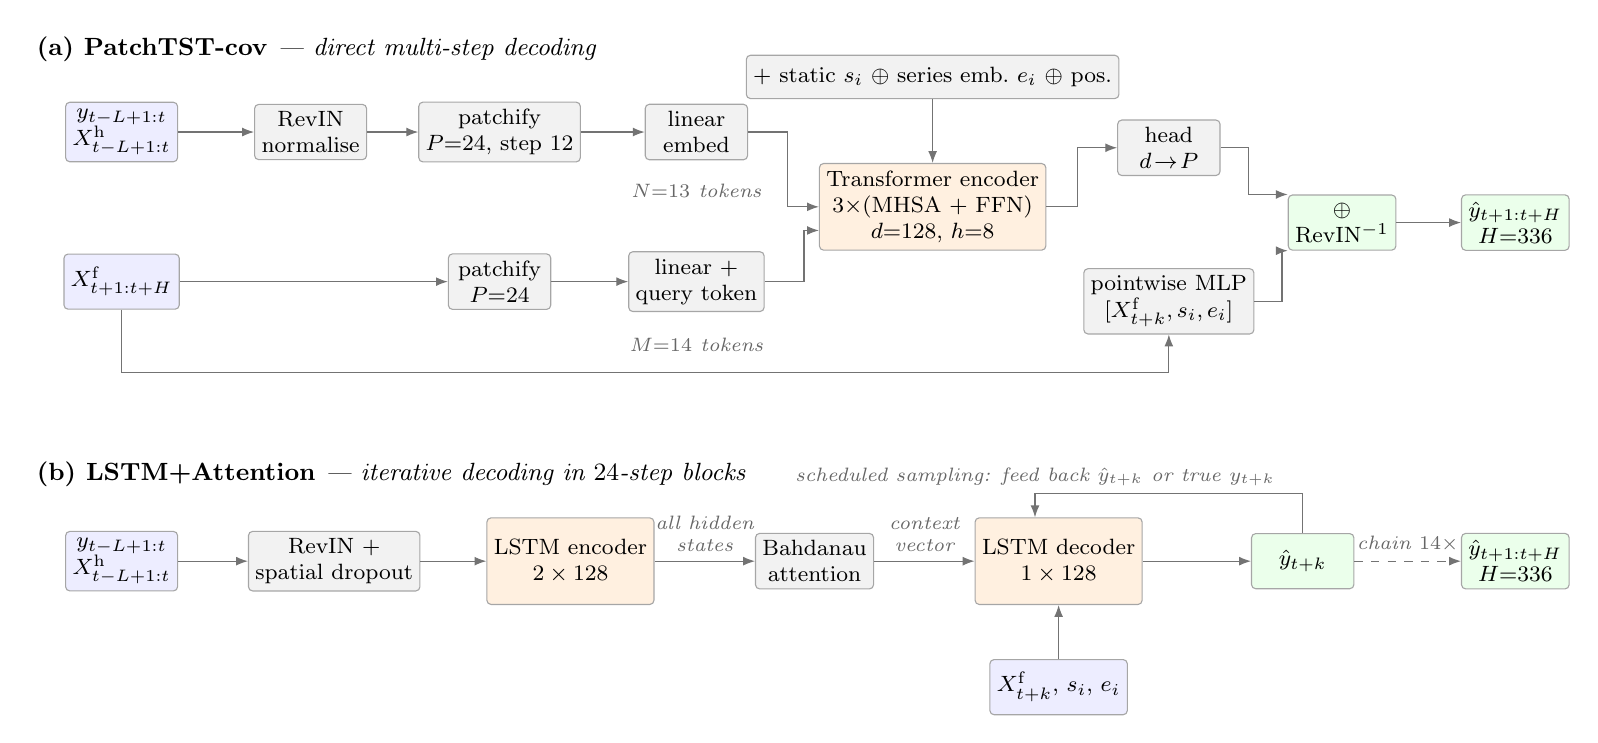
\begin{tikzpicture}[
  font=\footnotesize,
  box/.style={draw=black!35,rounded corners=1.5pt,align=center,inner sep=2.5pt,
              minimum height=7mm,minimum width=13mm},
  data/.style={box,fill=blue!7},
  op/.style={box,fill=black!5},
  core/.style={box,fill=orange!12,minimum height=11mm},
  res/.style={box,fill=green!8},
  arr/.style={-{Latex[length=1.5mm]},draw=black!55},
  lbl/.style={font=\scriptsize\itshape,text=black!60,align=center},
  panel/.style={font=\small\bfseries,anchor=west}
]
% ---------- (a) PatchTST-cov: direct decoding ----------
\node[panel] at (-0.6,3.1) {(a) PatchTST-cov \textmd{\itshape --- direct multi-step decoding}};
\node[data] (hist)  at (0.6,2.05) {$y_{t-L+1:t}$\\$X^{\mathrm{h}}_{t-L+1:t}$};
\node[data] (fut)   at (0.6,0.15) {$X^{\mathrm{f}}_{t+1:t+H}$};
\node[op]   (revin) at (3.0,2.05) {RevIN\\normalise};
\node[op]   (patchh) at (5.4,2.05) {patchify\\$P{=}24$, step $12$};
\node[op]   (patchf) at (5.4,0.15) {patchify\\$P{=}24$};
\node[op]   (embh)  at (7.9,2.05) {linear\\embed};
\node[op]   (embf)  at (7.9,0.15) {linear $+$\\query token};
\node[lbl]  (nh) at (7.9,1.30) {$N{=}13$ tokens};
\node[lbl]  (nf) at (7.9,-0.65) {$M{=}14$ tokens};
\node[core] (enc)   at (10.9,1.10)
  {Transformer encoder\\$3\times$(MHSA $+$ FFN)\\$d{=}128$, $h{=}8$};
\node[op,minimum height=5.5mm,minimum width=44mm] (stat) at (10.9,2.75)
  {$+$ static $s_i$ $\oplus$ series emb.\ $e_i$ $\oplus$ pos.};
\node[op]   (head)  at (13.9,1.85) {head\\$d\!\to\!P$};
\node[op]   (pw)    at (13.9,-0.10) {pointwise MLP\\$[X^{\mathrm{f}}_{t+k},s_i,e_i]$};
\node[res]  (sum)   at (16.1,0.90) {$\oplus$\\RevIN$^{-1}$};
\node[res]  (yhat)  at (18.3,0.90) {$\hat{y}_{t+1:t+H}$\\$H{=}336$};
\draw[arr] (hist) -- (revin);
\draw[arr] (revin) -- (patchh);
\draw[arr] (patchh) -- (embh);
\draw[arr] (fut) -- (patchf);
\draw[arr] (patchf) -- (embf);
\draw[arr] (embh.east) -- ++(0.5,0) |- (enc.west);
\draw[arr] (embf.east) -- ++(0.5,0) |- ([yshift=-3mm]enc.west);
\draw[arr] (stat) -- (enc);
\draw[arr] (enc.east) -- ++(0.4,0) |- (head.west);
\draw[arr] (fut.south) -- ++(0,-0.8) -| (pw.south);
\draw[arr] (head.east) -- ++(0.35,0) |- (sum.north west) ;
\draw[arr] (pw.east) -- ++(0.35,0) |- (sum.south west);
\draw[arr] (sum) -- (yhat);
% ---------- (b) LSTM + Attention: iterative decoding ----------
\begin{scope}[yshift=-3.75cm]
\node[panel] at (-0.6,1.45) {(b) LSTM+Attention \textmd{\itshape --- iterative decoding in $24$-step blocks}};
\node[data] (hist2) at (0.6,0.35) {$y_{t-L+1:t}$\\$X^{\mathrm{h}}_{t-L+1:t}$};
\node[op]   (sd)    at (3.3,0.35) {RevIN $+$\\spatial dropout};
\node[core] (encl)  at (6.3,0.35) {LSTM encoder\\$2\times128$};
\node[op]   (att)   at (9.4,0.35) {Bahdanau\\attention};
\node[core] (decl)  at (12.5,0.35) {LSTM decoder\\$1\times128$};
\node[data] (fut2)  at (12.5,-1.25) {$X^{\mathrm{f}}_{t+k},\,s_i,\,e_i$};
\node[res]  (yk)    at (15.6,0.35) {$\hat{y}_{t+k}$};
\node[res]  (blocks) at (18.3,0.35) {$\hat{y}_{t+1:t+H}$\\$H{=}336$};
\draw[arr] (hist2) -- (sd);
\draw[arr] (sd) -- (encl);
\draw[arr] (encl) -- node[lbl,above,pos=0.5]{all hidden\\states} (att);
\draw[arr] (att) -- node[lbl,above,pos=0.5]{context\\vector} (decl);
\draw[arr] (fut2) -- (decl);
\draw[arr] (decl) -- (yk);
\draw[arr] (yk.north) -- ++(0,0.5) -|
  node[lbl,above,pos=0.55]{scheduled sampling: feed back $\hat{y}_{t+k}$ or true $y_{t+k}$}
  ([xshift=-3mm]decl.north);
\draw[arr,dashed] (yk) -- node[lbl,above,pos=0.5]{chain $14\times$} (blocks);
\end{scope}
\end{tikzpicture}}
\caption{The two architectures. (a) \textbf{PatchTST-cov} patches the target history
\emph{and} the known-future covariates and lets one encoder attend over both; the
head reads the horizon off the query tokens (a direct $336$-step forecast) and a
pointwise MLP on $X^{\mathrm{f}}$ restores the resolution patching discards. (b)
\textbf{LSTM+Attention} decodes $24$ steps at a time and chains blocks. Both share
the static/series embedding and the raw-scale $L_1$ objective; the RevIN stage is
removed in the final models (Sec.~\ref{sec:ablations}).}
\label{fig:arch}
\end{figure*}

\subsection{PatchTST-cov}

The backbone follows PatchTST \cite{nie2023patchtst}: the RevIN-normalised target
history is cut into overlapping patches of length $P=24$ with stride $12$, giving
$N=13$ tokens, each linearly embedded to $d=128$. Channel independence is
preserved in the sense of the original paper --- one shared backbone sees a single
univariate target channel and every series is an independent sample. Encoder
covariates are fused into the history tokens by flattening the corresponding
$P\times F_{\mathrm{h}}$ block and projecting it to $d$.

The extension is on the decoder side (Fig.~\ref{fig:arch}a). We patch the
known-future covariates into $M = H/P = 14$ non-overlapping blocks, embed each,
add a learned query token, and \emph{append} them to the same token sequence.
Self-attention then relates every forecast segment both to the observed history
and to the other forecast segments, and a shared head maps each query token's
output to its $P$ target values. The forecast is therefore \textbf{direct}: no
autoregression inside the horizon, hence no error accumulation.

A patch token compresses $24$ hours of covariates into one $128$-dimensional vector
before the head expands it back to $24$ predictions, discarding within-patch
resolution. Because the drivers act largely instantaneously, we add a
\emph{pointwise residual path}: a two-layer MLP applied independently at each
forecast step to $[X^{\mathrm{f}}_{t+k}, s_i, e_i]$, summed onto the patch
prediction in normalised space, so the Transformer models only the residual
cross-step structure. This is the largest departure from our expos\'e's plan.

\subsection{LSTM+Attention}

The recurrent branch (Fig.~\ref{fig:arch}b) is the encoder--decoder from the
expos\'e, adapted to covariates. A two-layer LSTM ($128$ units) encodes
$[\text{RevIN}(y), X^{\mathrm{h}}, s_i, e_i]$ after spatial dropout; a
single-layer LSTM decoder unrolls $24$ steps, at each step consuming the known
covariates of the step being predicted, an additive attention context over all
encoder states \cite{bahdanau2015attention}, and either its own previous
prediction or the ground truth with probability $\epsilon$. We anneal $\epsilon$
linearly from $0.9$ to $0.1$ across training \cite{bengio2015scheduled}. Horizons
beyond one block are covered by chaining: predictions are appended to the
conditioning window together with the known covariates of those steps, and the
window is trimmed back to $L$.

\subsection{Ensemble, training and the gap}

The two families make structurally different errors, so we blend their rollouts
before clipping, with weights from greedy forward selection with replacement
\cite{caruana2004ensemble}. Which split that selection runs on turns out to matter
more than the values it returns, and Sec.~\ref{sec:ablations} returns to it.
Members are trained separately with AdamW ($\text{lr}=10^{-3}$, weight decay
$10^{-4}$), gradient clipping at $1.0$, batch size $64$, cosine annealing with warm
restarts \cite{loshchilov2017sgdr} and $L_1$ loss. Training windows are cut with a
stride that trades epoch cost against coverage: the shipped members use $2$--$6$
(PatchTST-cov, up to $151$k windows per epoch) and $6$--$12$ (LSTM, up to $55$k).
Predictions are clipped from below at the smallest target seen in training, since
the load index is strictly positive.

At private evaluation the input directory provides only the test covariates and the
forecast index, and the last \emph{released} target lies $336$ steps earlier. Our
checkpoint therefore bundles a $504$-step tail of the public history (with targets)
plus the public validation covariates; \texttt{predict.py} rebuilds one continuous
per-series timeline and rolls forward to the end of the requested index --- two
chained $336$-step blocks for PatchTST-cov, $28$ for the LSTM.

\section{Experiments on the benchmark}
\label{sec:experiments}

\subsection{Protocol}
\label{sec:protocol}

The public release contains no validation labels, so \emph{every} number we report
comes from a chronological split of \texttt{train.csv} ($96$ series
$\times$ $4{,}320$ hourly steps, 2023-01-01 to 2023-06-29), whose last $672$ steps
are held out and split in two. The \textbf{validation regime} scores steps
$3{,}649$--$3{,}984$ with the forecast origin at the end of the fit slice,
mirroring the public leaderboard; the \textbf{test regime} scores steps
$3{,}985$--$4{,}320$ from the \emph{same} origin, so the model must first bridge
$336$ unobserved steps, mirroring the private split. Model selection --- early
stopping, blend weights, all hyperparameters --- uses the validation regime only;
the test regime is scored once per final checkpoint. The evaluation \emph{set} is a
held-out tail rather than the hidden validation split, so these values are not
directly comparable to leaderboard scores, but in practice they track it: the
protocol predicted our leaderboard WAPE to within $0.05$.

\paragraph{Two compute budgets.} We report two, because the difference between them
turned out to be a first-order effect. The \textbf{constrained} budget is what a CPU
allows: a coarse window stride, so each epoch sees a few per cent of the available
windows. The \textbf{full} budget is a $26$-configuration grid on one RTX 2080 Ti at
strides $2$--$12$, up to $151$k windows per epoch. The ablations
(Sec.~\ref{sec:ablations}) use the full budget too.

\subsection{Main results}

\begin{table}[t]
\centering
\caption{Benchmark results on the held-out tails of \texttt{train.csv}; lower is
better, WAPE is the leaderboard's primary metric, and the test regime starts $336$
steps after the conditioning window. Each architecture appears twice, at the two
training budgets of Sec.~\ref{sec:protocol}; the parenthesised count is training
windows per epoch. $^{\ast}$ marks the variants that entered the shipped blend;
full six-metric tables are in \texttt{results/}.}
\label{tab:benchmark}
\scriptsize
\setlength{\tabcolsep}{1.8pt}
% generated by scripts/make_report_tables.py
\begin{tabular}{@{}lrrrr@{}}
\toprule
& \multicolumn{2}{c}{Validation} & \multicolumn{2}{c}{Test (gap)} \\
\cmidrule(lr){2-3}\cmidrule(lr){4-5}
Method & MAE & WAPE & MAE & WAPE \\
\midrule
Naive last value & 4.91 & 52.34 & 5.34 & 49.96 \\
Seasonal naive, lag 24 & 5.37 & 57.18 & 4.94 & 46.26 \\
Seasonal naive, lag 168 & 5.15 & 54.88 & 4.56 & 42.74 \\
Seasonal mean, dow$\times$hour & 3.50 & 37.27 & 3.35 & 31.38 \\
\midrule
LSTM+Attention (7k win.) & 1.73 & 18.42 & 2.57 & 24.09 \\
LSTM+Attention (no RevIN, 55k win.)$^{\ast}$ & 1.24 & 13.16 & 1.34 & 12.58 \\
PatchTST-cov (13k win.) & 1.49 & 15.92 & 1.66 & 15.56 \\
PatchTST-cov (no RevIN, 151k win.)$^{\ast}$ & 1.31 & 13.93 & 1.44 & 13.52 \\
\textbf{Blend of 5 runs (submitted)} & 1.21 & \textbf{12.91} & 1.32 & \textbf{12.40} \\
\bottomrule
\end{tabular}

\end{table}

Table~\ref{tab:benchmark} collects the results. Every model clears the mandatory
naive last-value reference and the stronger seasonal-mean baseline by a wide
margin; our submitted blend of \ensMembers{} runs reaches \ensValWape\,\% WAPE in
the validation regime against \seasonalValWape\,\% for the seasonal mean and
\naiveValWape\,\% for the naive baseline, and \ensTestWape\,\% in the gap regime
--- a \ensVsNaive\,\% error reduction over the reference we are required to beat.
The paired rows are the interesting part: each pair is one architecture under two
budgets, and they carry the two results that forced us to revise our conclusions.

\paragraph{The compute budget, not the architecture, decided our first comparison.}
Our expos\'e asked whether direct multi-step output beats iterative decoding. Under
the constrained budget --- $7$k windows per epoch for the LSTM, $13$k for the
Transformer --- the answer looked decisive: the Transformer reached
\patchRevinValWape\,\% while the recurrent model managed only \lstmRevinValWape\,\%
and collapsed to \lstmRevinTestWape\,\% across the gap. Re-run at the full budget,
with $8\times$ and $12\times$ the windows, the ranking \emph{inverts}: the LSTM
reaches \lstmValWape\,\% and the Transformer \patchValWape\,\%. Neither number was
a property of the architecture; both were properties of how starved it was. The
failure modes were in fact opposite, which is why no single budget separates them
fairly: the recurrent model was under-trained (its best epoch was always its last),
while the Transformer was already overfitting (best epoch $3$--$6$ of $40$--$60$).
The fix for one is the opposite of the fix for the other --- more data per epoch for
the LSTM, more dropout for the Transformer, worth $14.55 \rightarrow$
\patchValWape\,\%. We report it because ``patch Transformers beat recurrent models
here'' is a conclusion our own first experiment would have supported and our second
refutes.

\paragraph{The gap-regime collapse was a normalisation bug, not error
accumulation.} The same starved comparison also appeared to confirm that iterative
decoding accumulates error: the LSTM lost $5.7$ WAPE chaining $28$ blocks instead
of $14$. Sec.~\ref{sec:ablations} traces almost all of it to RevIN, and
Fig.~\ref{fig:horizon} shows the mechanism: fitting a line to MAE against the
forecast step, the pre-repair model drifts upward by $+0.26$ MAE per $100$ steps
while the repaired LSTM, the Transformer and their blend drift by $+0.02$ --- an
order of magnitude apart, and flat to within the noise of the curve.

\paragraph{Blending pays because the failure modes differ.} With both families
repaired and properly trained they land within $0.8$ WAPE of each other while
making differently-shaped errors, so the greedy selection of Sec.~\ref{sec:ablations}
over five runs beats its own best member by $0.25$ WAPE.

\begin{figure}[t]
\centering
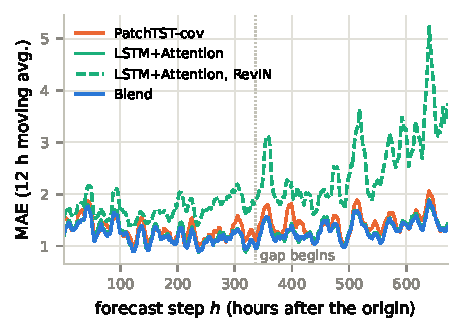
\includegraphics[width=\columnwidth]{figures/error_by_horizon.pdf}
\caption{MAE against the forecast step $h$ ($12$-hour moving average). The two
held-out windows share one origin and are contiguous, so $h=1\dots336$ is the
validation regime and $h=337\dots672$ the test regime. Only the pre-repair
recurrent model (dashed) drifts upward with $h$. Fitted drift per $100$ steps:
$+0.258$ MAE with RevIN versus $+0.020$ (LSTM), $+0.025$ (PatchTST-cov) and
$+0.022$ (blend) without it.}
\label{fig:horizon}
\end{figure}

\subsection{Ablations and analysis}
\label{sec:ablations}

\begin{table}[t]
\centering
\caption{Ablations at the full budget. Both references are the shipped
configuration --- RevIN-free, stride $6$, $40$/$30$ epochs --- and reproduce their
Table~\ref{tab:benchmark} rows exactly, so every $\Delta$ answers ``what if I
change this one thing about the submitted model''. RevIN is therefore \emph{added}
rather than removed. Positive $\Delta$ is worse. ``No future cov.\ tokens'' also
removes the pointwise path.}
\label{tab:ablations}
\scriptsize
\setlength{\tabcolsep}{4pt}
% generated by scripts/make_report_tables.py
\begin{tabular}{lrrrr}
\toprule
& \multicolumn{2}{c}{Validation} & \multicolumn{2}{c}{Test (336\,h gap)} \\
\cmidrule(lr){2-3}\cmidrule(lr){4-5}
Configuration & WAPE & $\Delta$ & WAPE & $\Delta$ \\
\midrule
PatchTST-cov (ref.) & 14.76 & & 13.68 & \\
\quad $+$ RevIN & 15.08 & +0.32 & 14.45 & +0.77 \\
\quad MSE instead of $L_1$ & 15.23 & +0.47 & 14.07 & +0.39 \\
\quad no covariates (vanilla) & 33.55 & +18.80 & 32.65 & +18.97 \\
\quad no future cov.\ tokens & 33.42 & +18.66 & 30.36 & +16.68 \\
\quad no pointwise path & 15.36 & +0.61 & 14.38 & +0.70 \\
\quad no series embedding & 15.22 & +0.46 & 14.37 & +0.69 \\
\quad patch 48, step 24 & 14.55 & -0.21 & 13.87 & +0.19 \\
\quad patch 8, step 4 & 14.31 & -0.45 & 13.35 & -0.33 \\
\midrule
LSTM+Attention (ref.) & 13.16 & & 12.58 & \\
\quad $+$ RevIN & 15.99 & +2.83 & 17.38 & +4.80 \\
\quad free running only & 13.53 & +0.37 & 12.81 & +0.24 \\
\quad no attention & 13.30 & +0.14 & 12.61 & +0.03 \\
\quad no covariates & 33.73 & +20.57 & 39.14 & +26.57 \\
\quad no series embedding & 17.27 & +4.11 & 24.33 & +11.75 \\
\quad teacher forcing only & 14.14 & +0.98 & 13.51 & +0.94 \\
\bottomrule
\end{tabular}

\end{table}

\paragraph{The covariate contract dominates everything else.} Removing the future
covariate tokens costs $18.7$ WAPE points and removing the covariates entirely
$18.8$; the recurrent model loses $20.6$ the same way, $26.6$ across the gap. No
other edit in Table~\ref{tab:ablations} moves either model by more than $4.2$, and
most by less than $1$. This is the empirical core of the paper: the backbone is not
what produces the accuracy --- the availability of future covariates is --- and the
architecture's job is to consume them at the right resolution.

\paragraph{RevIN hurts both families.} Adding it back costs the Transformer
$+0.32$/$+0.77$ and the recurrent model $+2.83$/$+4.80$; the asymmetry is the clue.
RevIN re-injects the conditioning window's own mean and standard deviation into the
prediction, and over $336$--$672$ steps last week's level is a poor estimate of next
fortnight's, so the transform adds variance rather than removing shift. For the
\emph{iterative} decoder it is worse: every chained block re-estimates those
statistics \emph{from the block it just predicted}, so a level error re-enters the
normaliser and is amplified at each of the $28$ hops --- the mechanism behind the
collapse we first attributed to iterative decoding. The sign is the same on
validation, so we could act on it without consulting the test split; no member of
the shipped blend uses RevIN.

\paragraph{Two components swapped places when we stopped starving the models.} We
first ran this table at a $16\times$ coarser stride, and two rows read very
differently there. \emph{Attention} looked load-bearing for the recurrent branch
($+11.03$ without it); at the full budget it is worth $+0.14$/$+0.03$ --- nothing.
\emph{The per-series embedding} looked worthless ($-0.12$, within noise); at the
full budget it is the most valuable thing the LSTM has after the covariates,
$+4.11$/$+11.75$. Both reversals point the same way as the architecture comparison
in Sec.~\ref{sec:experiments}: a starved model cannot exploit capacity, so
components that supply capacity look useless and their substitutes look essential.
The starved numbers were not merely noisier, they were misleading in a systematic
direction. The embedding result also settles a question from our expos\'e --- the
per-unit response the OLS diagnostic predicted is real, but the Transformer absorbs
it through the covariate pathway ($+0.46$/$+0.69$) while the recurrent decoder,
seeing one step at a time, needs it stated explicitly.

\paragraph{Scheduled sampling helps, and couples the schedule to the budget.}
Both endpoints of the anneal are worse than the anneal itself: teacher forcing only
($\epsilon=1$) costs $+0.98$/$+0.94$ --- the classic exposure-bias failure --- and
free running only ($\epsilon=0$) costs $+0.37$/$+0.24$. The schedule has a side
effect we did not anticipate, though: $\epsilon$ is annealed across the
\emph{whole} epoch budget, so a longer budget is not a superset of a shorter one but
a slower anneal. Stretching the winning $30$-epoch LSTM to $100$ epochs made it
\emph{worse} ($13.16 \rightarrow 13.40$), and the usual guard --- more epochs cannot
hurt, early stopping will catch it --- fails when the objective itself moves with
the epoch index. Finally, replacing $L_1$ with MSE costs $+0.47$/$+0.39$ under WAPE,
as the metric-alignment argument of Sec.~\ref{sec:method} predicts.

\paragraph{Where the design is not optimal.} Halving the patch to $P=8$ improves
both regimes ($-0.45$/$-0.33$), so the length we inherited from PatchTST is not the
right one here --- unsurprising, since finer patches do the same job as the
pointwise residual path ($+0.61$/$+0.70$), which exists precisely because $P=24$
discards within-patch resolution. We report it rather than quietly adopting it: it
arrived after the blend was built, and acting on it now would be tuning on the
split we report.

\paragraph{Blend weights are chosen on a gap-matched criterion.} \emph{Which} split
the greedy selection runs on matters more than the weights it returns: a weight
tuned on the validation regime is tuned on a regime the private split never runs
in. We therefore select on a \emph{gap-matched} criterion --- the same labels, but
with the origin moved back one window so members must bridge $336$ unobserved steps
first (\gapValWape\,\% for the blend, against \ensValWape\,\% ungapped). With
RevIN-free members the two criteria agree; before the repair they did not, because
RevIN's damage is invisible without a gap. The weights land on $0.36/0.24/0.12$ over
three LSTM runs and $0.24/0.04$ over two PatchTST runs --- and those two Transformers
are individually the \emph{weakest} in the pool ($13.93$ and $14.55$ against
$13.16$), so the blend buys decorrelated errors, not accuracy.

\paragraph{What the model uses.} Shuffling one covariate at a time across the
forecast window gives a concentrated ranking: from a base of \patchValWape\,\%,
\texttt{queue\_pressure\_forecast} alone is worth $+15.9$ WAPE and
\texttt{network\_pressure\_forecast} $+8.7$, then \texttt{maintenance\_known}
($+4.5$), \texttt{demand\_forecast} ($+3.0$) and \texttt{promotion\_intensity}
($+2.3$); nothing else reaches $+2.0$ and the calendar encodings are negligible
($\le +0.26$). Two of the $19$ covariates carry most of the accuracy. The values
are a per-channel lower bound, since the covariates are correlated; the full
ranking is in \texttt{figures/permutation\_importance.pdf}.

\section{Additional dataset: Jena Climate}
\label{sec:jena}

\paragraph{Dataset and use case.} The Jena Climate dataset \cite{jena2026} records
$14$ atmospheric variables --- pressure, air and potential temperature, dew point,
humidity, three vapour-pressure channels, air density, wind speed and direction ---
every $10$ minutes at the Max Planck Institute for Biogeochemistry weather station,
2009-01-01 to 2017-01-01 ($420{,}551$ rows). The use case is local weather
nowcasting: the next two weeks of temperature, and of pressure as a second target,
from the recent multivariate state.

We chose it because it \emph{inverts} the benchmark's covariate contract --- nothing
except the calendar is known in advance --- so it tests whether our gains come from
modelling or from unusually generous inputs. It is also harder as a multivariate
problem: the channels are non-linearly coupled (dew point and vapour pressure are
functions of temperature and humidity) and the target has diurnal \emph{and} annual
seasonality, the latter longer than any window we condition on.

\paragraph{What had to change.} Exactly one abstraction: a \emph{past-only}
covariate group. Encoder features become $[\text{known-future} \cup
\text{past-only}]$ while decoder features are the known-future subset alone, so
$F_{\mathrm{h}}=24 > F_{\mathrm{f}}=8$; both architectures read the two widths from
the specification and no layer was rewritten. When the iterative decoder appends a
predicted block to its window it cannot know the past-only channels there, so they
are filled by persistence --- never by their true values, which would leak the
answer. Preprocessing is dataset-specific: hourly means, repair of the $-9999$ wind
sentinel, Cartesian wind components, day-of-year sine/cosine. The split is
chronological $70/10/20$, scored rolling-origin (one origin every $336$ steps);
temperature crosses zero, so we report MAE rather than WAPE.

\begin{table}[t]
\centering
\caption{Jena Climate, hourly, $L=168$, $H=336$, rolling-origin evaluation.
Temperature crosses zero, so MAE replaces WAPE; RMSE is in
\texttt{results/jena.json}. Both targets use the same architecture and optimiser
settings as the benchmark, with a reduced epoch budget and no static or missingness
features; the calendar encodings are the only known-future covariates.}
\label{tab:jena}
\scriptsize
\setlength{\tabcolsep}{3pt}
% generated by scripts/make_report_tables.py
\begin{tabular}{lrrrr}
\toprule
& \multicolumn{2}{c}{temperature [$^{\circ}$C]} & \multicolumn{2}{c}{pressure [mbar]} \\
\cmidrule(lr){2-3}\cmidrule(lr){4-5}
Method (MAE) & val & test & val & test \\
\midrule
Naive last value & 3.79 & 5.96 & 8.04 & 7.88 \\
Seasonal naive, lag 24 & 3.53 & 5.00 & 8.59 & 8.09 \\
Seasonal mean & 5.56 & 6.69 & 6.73 & 6.49 \\
\midrule
PatchTST-cov (ours) & 3.04 & 3.76 & 7.23 & 6.42 \\
LSTM+Attention (ours) & 2.94 & 3.79 & 8.19 & 7.00 \\
\bottomrule
\end{tabular}

\end{table}

\paragraph{Does it transfer?} Only partly, and where it fails is the useful result
(Table~\ref{tab:jena}). On \emph{temperature} it transfers cleanly: both models
beat every baseline on both splits, cutting test MAE from $5.00$ to $3.76$, a
$25$\,\% reduction, with no tuning beyond the feature specification. On
\emph{pressure} it essentially fails: PatchTST-cov is worse than the seasonal mean
on validation ($7.23$ vs $6.73$) and only ties it on test, and the recurrent model
loses on both.

The contrast is what our thesis predicts. With only the calendar known in advance,
the query tokens and the pointwise path have almost no input and the model falls
back on target history --- precisely the regime in which linear baselines are
competitive \cite{zeng2023dlinear}. What survives then depends on how much of the
target that history explains: temperature has a diurnal cycle the encoder can
exploit, whereas pressure is driven by synoptic systems invisible in a $168$-hour
window and whose long-run mean the seasonal baseline already captures. The two
decoders are again within $0.03$ MAE on temperature, a third sign that the
direct/iterative choice is not what separates models. Backbone, recipe and
past-only abstraction transfer unchanged; the \emph{size} of the win moves with the
covariate contract.

\section{Conclusion}

We set out to compare a recurrent-attention hybrid against a patch Transformer, and
the most useful results were not about which backbone wins. Because the benchmark
supplies all $22$ covariates for the forecast window, the task is
covariate-conditioned regression rather than extrapolation, and consuming that
window at the right resolution accounts for essentially the whole improvement:
every other component in Table~\ref{tab:ablations} is worth an order of magnitude
less, attention itself worth $+0.14$.

Our other results are corrections to conclusions we had already drawn. The
gap-regime collapse we would have reported as evidence for direct decoding was
RevIN compounding through the rollout. And three rankings --- the two architectures,
attention against none, the per-series embedding against none --- came out
differently once the models were no longer starved, always in the same direction:
starvation makes capacity look useless and its substitutes essential. A blend of
\ensMembers{} runs reaches \ensTestWape\,\% WAPE across the gap and
\ensPublicWape\,\% on the public leaderboard, within $0.09$ of what our local
protocol predicted --- which is the real result here: the protocol, not any one
number.

\paragraph{Limitations.} Selection rests on a single $336$-step validation window
with few seed repeats; re-scoring identical checkpoints under a different thread
count moves WAPE by up to $0.07$, so differences below $\approx0.1$ are not real
and the top three blend members sit inside that band. Every ablation is a single
run, and having watched two of them reverse with the budget we would not defend any
$\Delta$ under $\approx0.5$ without seeds. The gap handling assumes the private
window is contiguous with the public history. Finally the model is deterministic
and trained on $L_1$, hence predicts a conditional median: on this right-skewed
target it under-predicts the total by $\approx7$\,\% by construction, optimal for
WAPE and wrong for anything volume-based. A quantile head
\cite{salinas2020deepar} is the principled fix; a finer patch
(Sec.~\ref{sec:ablations}), cross-series attention over the $96$ units and an MLP
covariate baseline such as TiDE \cite{das2023tide} are what we would try next.

\section*{Contributions}
\small

\textbf{Rosela Berberi} --- covariate-contract analysis; feature pipeline;
PatchTST-cov; training and evaluation harness including the gap-aware protocol;
inference and submission packaging. \textbf{Anja Koroveshi} --- LSTM+Attention
including the RevIN statefulness fix, scheduled sampling and the chained rollout;
baselines and metrics; ablation and permutation studies; Jena Climate; figures.
Experiments were designed and the report written jointly.

\bibliographystyle{plain}
\bibliography{references}

\end{document}
